%%%%%%%%%%%%%%%%%%%%%%%%%%%%%%%%%%%%%%%%%%%%%%%%%%%%
% Document type, global settings, and packages
%%%%%%%%%%%%%%%%%%%%%%%%%%%%%%%%%%%%%%%%%%%%%%%%%%%%

\documentclass[11pt,twoside]{report}   %12 point font for Times New Roman
\usepackage{graphicx}  %for images and plots
\usepackage[a4paper,hmargin=3.5cm,vmargin=5.3cm,head=1.5cm,foot=3.2cm]{geometry}
\usepackage{setspace}   %use this package to set linespacing as desired
\doublespacing
\usepackage{times}      %set Times New Roman as the font
\usepackage[explicit]{titlesec}  %title control and formatting
\usepackage[titles]{tocloft}  %table of contents control and formatting
\usepackage[backend=biber,sorting=none,bibstyle=phys]{biblatex}  %reference manager
\usepackage[bookmarks=true, hidelinks]{hyperref}
\usepackage[page]{appendix}  %for appendices
\usepackage[figuresright]{rotating}  %for rotated, landscape images
\usepackage[normalem]{ulem}  %for underlined section titles
% \usepackage[english,dutch]{babel}    % i18n

% \usepackage{bold-extra} % include bold and cap\usepackage[dutch,english]{babel}

% https://tex.stackexchange.com/questions/47576/combining-ifxetex-and-ifluatex-with-the-logical-or-operation
\usepackage{ifxetex,ifluatex}
\newif\ifxetexorluatex
\ifxetex
  \xetexorluatextrue
\else
  \ifluatex
    \xetexorluatextrue
  \else
    \xetexorluatexfalse
  \fi
\fi

\ifxetexorluatex
  % \usepackage{stix}
  \usepackage{fontspec}
  \usepackage{unicode-math}
  % \setsansfont{CMU Sans Serif}%{Arial}
  % \setmainfont{CMU Serif}%{Times New Roman}
  % \setmonofont{CMU Typewriter Text}%{Consolas}
  % \defaultfontfeatures{Ligatures={TeX}}
  \defaultfontfeatures{Scale=MatchLowercase,Ligatures=TeX}
  % \setmainfont{STIX Two Text}
  \setmainfont{Noto Serif}
  \setmathfont{TeX Gyre Schola Math}
  % https://gist.github.com/dlimpid/5454229
  \usepackage{xeCJK}
  \xeCJKsetup{%
    CJKspace=true,% % true이면 띄어쓰기 사용. 중국어, 일어는 필요 없을수도
    % CJKmath=true,%  % true면 math environment 안에서 CJK 글자 사용
    CJKecglue={}%   % Western과 CJK 사이의 공백 지정: {}로 간격을 없앰
  }
  \setCJKmainfont[
    Path=fonts/,
    Extension=.otf,
    BoldFont=NotoSerifCJKkr-Bold,
    AutoFakeSlant,
    Ligatures=TeX]{NotoSerifCJKkr-Regular.otf}
  \setCJKsansfont[
    Path=fonts/,
    Extension=.otf,
    BoldFont=NotoSerifCJKkr-Bold,
    AutoFakeSlant,
    Ligatures=TeX]{NotoSerifCJKkr-Regular.otf}
  \setCJKmonofont[
    Path=fonts/,
    Extension=.otf,
    BoldFont=NotoSerifCJKkr-Bold,
    AutoFakeSlant,
    Ligatures=TeX]{NotoSerifCJKkr-Regular.otf}
  \usepackage[scale=0.8]{noto-mono}
  \setmonofont{Noto Sans Mono}
  % small url fonts
  \renewcommand{\UrlFont}{\ttfamily\small}
\else
  \usepackage{amssymb,amsmath}
  \usepackage[T2A,T1]{fontenc}
  \usepackage[utf8]{inputenc}
  \usepackage{kotex}
  \usepackage{textcomp} % provide euro and other symbols
\fi

\ifxetex
  \XeTeXinputnormalization=1
\fi

\renewcommand{\floatpagefraction}{0.1} % one figure in one page

\usepackage{url}          % simple URL typesetting
\usepackage{booktabs}     % proessional-quality tables
\usepackage{bookmark}
\usepackage{hyperref}     % hyperlinks
\usepackage{siunitx}		  % SI unit
\usepackage{multicol} 		% use multicol in table
\usepackage{multirow} 		% use multirow in table
\usepackage{xcolor}			  % color fonts
\usepackage{adjustbox}    % fit table to page width
\usepackage[noabbrev,nameinlink]{cleveref}		% for multiple cross-reference
\usepackage[super]{nth}		% th
\usepackage{afterpage}    % separate page for floats and tables
\usepackage{titlefoot}    % keywords on footnote
\usepackage[intoc]{nomencl}  % nomenclature
\makenomenclature
\setlength{\nomitemsep}{-\parsep}
\setlength{\nomlabelwidth}{1.7cm}

%%%%%%%%%%%%%%%%%%%%%%%%%%%%%%%%%%%
% Bibliography
%%%%%%%%%%%%%%%%%%%%%%%%%%%%%%%%%%%

%Add your bibliography file here
\addbibresource{references.bib}

% escape % in biber (perl program)
\DeclareSourcemap{
  \maps[datatype = bibtex]{
    \map{
       \step[fieldsource = abstract,
          match = \regexp{([^\\])\%},
          replace = \regexp{$1\\\%}]
    }
  }
}

% prevent certain fields in references from printing in bibliography
\AtEveryBibitem{\clearfield{issn}}
\AtEveryBibitem{\clearlist{issn}}

\AtEveryBibitem{\clearfield{language}}
\AtEveryBibitem{\clearlist{language}}

\AtEveryBibitem{\clearfield{doi}}
\AtEveryBibitem{\clearlist{doi}}

\AtEveryBibitem{\clearfield{url}}
\AtEveryBibitem{\clearlist{url}}

\AtEveryBibitem{%
  \ifentrytype{online}
    {}
    {\clearfield{urlyear}\clearfield{urlmonth}\clearfield{urlday}}}

% footnote for keywords in abstract
% https://tex.stackexchange.com/questions/30720/footnote-without-a-marker
\newcommand\blfootnote[1]{%
  \begingroup
  \renewcommand\thefootnote{}\footnote{#1}%
  \addtocounter{footnote}{-1}%
  \endgroup
}
%%%%%%%%%%%%%%%%%%%%%%
% Start of Document
%%%%%%%%%%%%%%%%%%%%%%

\begin{document}

%%%%%%%%%%%%%%%%%%%%%%%%%%%%%%%%%%%%%
% Cover Page
%%%%%%%%%%%%%%%%%%%%%%%%%%%%%%%%%%%%%

%% Define your thesis title, your name, your school, and your month and year of graduation here
\newgeometry{top=7.13cm,bottom=4.75cm,right=4.17cm,left=4.17cm}
\newcommand{\coverTitle}{Dissertation Title}
\newcommand{\coverName}{Name}

%%%%%%%%%%%%%%%%%%%%%%%%%%%%%%%%%%%%%%%%%%%%%%%%%%%%%%%%%
% Do not edit these lines unless you wish to customize
% the template
%%%%%%%%%%%%%%%%%%%%%%%%%%%%%%%%%%%%%%%%%%%%%%%%%%%%%%%%%

\begin{titlepage}
\clearpage\thispagestyle{empty}
\begin{center}

{\fontsize{20pt}{20pt} \selectfont \coverTitle \vspace{3.5cm} \par}

{\fontsize{16pt}{20pt} \selectfont \coverName \vspace{3.5cm} \par}
{\fontsize{16pt}{20pt} \selectfont
The Graduate School  \par
Yonsei University \par
Department of blahblah \par}
\vfill

\end{center}
\end{titlepage}



\currentpdfbookmark{Cover Page}{coverPage}  %add PDF bookmark for this page

%%%%%%%%%%%%%%%%%%%%%%%%%%%%%%%%%%%%%
% Title Page
%%%%%%%%%%%%%%%%%%%%%%%%%%%%%%%%%%%%%

% define title page margin
% \newgeometry{top=1in,bottom=1in,right=0.5in,left=1.5in}
%% Define your thesis title, your name, your school, and your month and year of graduation here
\newgeometry{top=4.75cm,bottom=3.56cm,right=4.17cm,left=4.17cm}

\newcommand{\thesisTitle}{Title}
\newcommand{\mythesisTitle}{Title}
\newcommand{\yourName}{Author Name}
\newcommand{\yourMonth}{June}
\newcommand{\yourYear}{2021}

%%%%%%%%%%%%%%%%%%%%%%%%%%%%%%%%%%%%%%%%%%%%%%%%%%%%%%%%%
% Do not edit these lines unless you wish to customize
% the template
%%%%%%%%%%%%%%%%%%%%%%%%%%%%%%%%%%%%%%%%%%%%%%%%%%%%%%%%%

\begin{titlepage}
\clearpage\thispagestyle{empty}
\begin{center}

{\fontsize{20pt}{20pt} \selectfont \mythesisTitle \vspace{3.56cm} \par}
{\fontsize{16pt}{16pt}
\selectfont
    A Dissertation Submitted to the \par
    Deparment of blahblah \par
    and the Graduate School of Yonsei University \par
    in partial fulfillment of the \par
    requirements for the degree of \par
    Doctor of Philosophy in Blahblah \\
    \vspace{3.56cm} 
    \par}

\begin{doublespacing}
    {\fontsize{16pt}{18pt}
    \selectfont 
    \vspace{0.95cm}
    \yourName \par
    \vspace{0.95cm}
    \yourMonth{} \yourYear{} \par
}
\vfill
\par

\end{doublespacing}
\end{center}
\end{titlepage}



\currentpdfbookmark{Title Page}{titlePage}  %add PDF bookmark for this page

%%%%%%%%%%%%%%%%%%%%%%%%%%%%%%%%%%%%%
% Approval Page
%%%%%%%%%%%%%%%%%%%%%%%%%%%%%%%%%%%%%

\newgeometry{top=4.15cm,bottom=4.15cm,right=4.17cm,left=4.17cm}
%% Define your committee members. If you have less than 6, simple delete/comment the unused lines
\newcommand{\approvalAuthor}{Author Name}
\newcommand{\committeeMemberOne}{Thesis Supervisor: Prof. Dr. Committee01}
\newcommand{\committeeMemberTwo}{Prof. Dr. Committee02}
\newcommand{\committeeMemberThree}{Prof. Dr. Committee03}
\newcommand{\committeeMemberFour}{Prof. Dr. Committee04}
\newcommand{\committeeMemberFive}{Prof. Dr. Committee05}

%%%%%%%%%%%%%%%%%%%%%%%%%%%%%%%%%%%%%%%%%%%%%%%%%%%%%%%%%
% Do not edit these lines unless you wish to customize
% the template
% Remove committeeMemberFour and committeeMembmerFive 
% if you are master student
%%%%%%%%%%%%%%%%%%%%%%%%%%%%%%%%%%%%%%%%%%%%%%%%%%%%%%%%%

\begin{titlepage}
\clearpage\thispagestyle{empty}

\begin{singlespacing}

\centering

\large{
	This certifies that the dissertation of \approvalAuthor is approved.
}

\vspace{2.97cm}		%adjust the number in front of "\baselineskip" for alignment

\par\rule{6.5cm}{0.8pt}\null \\
\large{\committeeMemberOne} \\
\vspace{1.78cm}

\par\rule{6.5cm}{0.8pt}\null \\
\large{\committeeMemberTwo} \\
\vspace{1.78cm}

\par\rule{6.5cm}{0.8pt}\null \\
\large{\committeeMemberThree} \\
\vspace{1.78cm}

\par\rule{6.5cm}{0.8pt}\null \\
\large{\committeeMemberFour} \\
\vspace{1.78cm}

\par\rule{6.5cm}{0.8pt}\null \\
% \par\parindent=7\baselineskip\hrulefill\null \\
\large{\committeeMemberFive} \\
\vspace{1.78cm}

{\fontsize{14pt}{24pt}
	\selectfont
	Graduate School \par
	Yonsei University \par
	June 2021 \par
}
\vfill
\end{singlespacing}
\end{titlepage}


%%%%%%%%%%%%%%%%%%%%%%%%%%%%%%%%%%%%%
% Acknowledgments
%%%%%%%%%%%%%%%%%%%%%%%%%%%%%%%%%%%%%

% \pagenumbering{roman}
% \addcontentsline{toc}{chapter}{Acknowledgments}
% \setcounter{page}{5} % set the page number appropriately based on the number of intro pages
\clearpage
\newgeometry{hmargin=3.5cm,vmargin=5.3cm,head=3.5cm,foot=3.2cm}
\begin{centering}
\textbf{ACKNOWLEDGEMENTS}\\
\vspace{\baselineskip}
\end{centering}

Lorem ipsum dolor sit amet, consectetur adipiscing elit, sed do eiusmod tempor incididunt ut labore et dolore magna aliqua. Ut enim ad minim veniam, quis nostrud exercitation ullamco laboris nisi ut aliquip ex ea commodo consequat. Duis aute irure dolor in reprehenderit in voluptate velit esse cillum dolore eu fugiat nulla pariatur. Excepteur sint occaecat cupidatat non proident, sunt in culpa qui officia deserunt mollit anim id est laborum.

\pagenumbering{gobble}
\thispagestyle{empty}
\clearpage


%\addtocontents{toc}{\cftpagenumbersoff{chapter}}

%\currentpdfbookmark{Acknowledgments}{acknowledgments}
%\addtocontents{toc}{\cftpagenumberson{chapter}}
% Set location of page numbering as just below text body
\newgeometry{hmargin=3.5cm,vmargin=5.3cm,head=1.5cm,foot=3.2cm,footskip=1cm}
%%%%%%%%%%%%%%%%%%%%%%%%%%%%%%%%%%%%%
% Table of Contents
%%%%%%%%%%%%%%%%%%%%%%%%%%%%%%%%%%%%%
\pagenumbering{roman}
\setcounter{page}{1} % set the page number appropriately based on the number of intro pages
% Format for Table of Contents
\renewcommand{\cftchapdotsep}{\cftdotsep}  %add dot separators
\renewcommand{\cftchapfont}{\bfseries}  %set title font weight
\renewcommand{\cftchappagefont}{}  %set page number font weight
\renewcommand{\cftchappresnum}{Chapter }
\renewcommand{\cftchapaftersnum}{:}
\renewcommand{\cftchapnumwidth}{6em}
\renewcommand{\cftchapafterpnum}{\vskip\baselineskip} %set correct spacing for entries in single space environment
\renewcommand{\cftsecafterpnum}{\vskip\baselineskip}  %set correct spacing for entries in single space environment
\renewcommand{\cftsubsecafterpnum}{\vskip\baselineskip} %set correct spacing for entries in single space environment
\renewcommand{\cftsubsubsecafterpnum}{\vskip\baselineskip} %set correct spacing for entries in single space environment

%format title font size and position (this also applys to list of figures and list of tables)
\titleformat{\chapter}[display]
{\normalfont\bfseries\filcenter}{\chaptertitlename\ \thechapter}{0pt}{\MakeUppercase{#1}}

\renewcommand\contentsname{Table of Contents}

\begin{singlespace}
\tableofcontents
\end{singlespace}

\currentpdfbookmark{Table of Contents}{TOC}

\clearpage

%%%%%%%%%%%%%%%%%%%%%%%%%%%%%%%%%%%%%
% List of figures and tables
%%%%%%%%%%%%%%%%%%%%%%%%%%%%%%%%%%%%%

\addcontentsline{toc}{chapter}{List of Tables}
\begin{singlespace}
	\setlength\cftbeforetabskip{\baselineskip}  %manually set spacing between entries
	\listoftables
\end{singlespace}

\clearpage

\addcontentsline{toc}{chapter}{List of Figures}
\begin{singlespace}
\setlength\cftbeforefigskip{\baselineskip}  %manually set spacing between entries
\listoffigures
\end{singlespace}

\clearpage

\printnomenclature
\clearpage

%%%%%%%%%%%%%%%%%%%%%%%%%%%%%%%%%%%%%%%%%%%%%%%%%%%%%%%%%%%%%%%%%
% This is the Abstract
%%%%%%%%%%%%%%%%%%%%%%%%%%%%%%%%%%%%%%%%%%%%%%%%%%%%%%%%%%%%%%%%%
\addcontentsline{toc}{chapter}{Abstract}
% \setcounter{page}{5} % set the page number appropriately based on the number of intro pages
\clearpage
\begin{centering}
\textbf{ABSTRACT}\\
\vspace{\baselineskip}
\end{centering}

\begin{flushright}
    Name  \\
    Department of ... \\
    The Graduate School, Yonsei University
\end{flushright}

Lorem ipsum dolor sit amet, consectetur adipiscing elit, sed do eiusmod tempor incididunt ut labore et dolore magna aliqua. Ut enim ad minim veniam, quis nostrud exercitation ullamco laboris nisi ut aliquip ex ea commodo consequat. Duis aute irure dolor in reprehenderit in voluptate velit esse cillum dolore eu fugiat nulla pariatur. Excepteur sint occaecat cupidatat non proident, sunt in culpa qui officia deserunt mollit anim id est laborum.

\blfootnote{Keywords: Keyword 1, Keyword 2, Keyword 3}
%\pagenumbering{gobble}  %remove page number on summary page




%%%%%%%%%%%%%%%%%%%%%%%%%%%%
%
% Remark
%
%%%%%%%%%%%%%%%%%%%%%%%%%%%%

\clearpage
\begin{centering}
\textbf{REMARK}\\
\vspace{\baselineskip}
\end{centering}

\vspace{\baselineskip}
Material from: 
\vspace{\baselineskip}

\begin{center}
\textbf{Some passages of this dissertation have been reprinted from the above sources.}
\end{center}


%%%%%%%%%%%%%%%%%%%%%%%%%%%%
%
% Chapters
%
%%%%%%%%%%%%%%%%%%%%%%%%%%%%

%%%%%%%%%%%%%%%%%%%%%%
% formatting
%%%%%%%%%%%%%%%%%%%%%%

% resume page numbering for rest of document
\clearpage
\pagenumbering{arabic}
\setcounter{page}{1} % set the page number appropriately

% Adjust chapter title formatting
\newcommand{\chapternamefont}{\scshape\Large}% Chapter name font
\newcommand{\chaptertitlefont}{\LARGE\bfseries}% Chapter title font
\titleformat{\chapter}[display]
{\normalfont\bfseries\chapternamefont\raggedright}{\MakeUppercase\chaptertitlefont\chaptertitlename\ \thechapter}{0pt}{\MakeUppercase{#1}}  %spacing between titles
\titlespacing*{\chapter}
  {0pt}{\topskip}{30pt}	%controls vertical margins on title

% Adjust section title formatting
\titleformat{\section}{\normalfont\bfseries}{\thesection}{1em}{#1}

% Adjust subsection title formatting
% \titleformat{\subsection}{\normalfont}{\uline{\thesubsection}}{0em}{\uline{\hspace{1em}#1}}
\titleformat{\subsection}{\normalfont\bfseries}{\thesubsection}{1em}{#1}

% Adjust subsubsection title formatting
\titleformat{\subsubsection}{\normalfont\itshape}{\thesubsection}{1em}{#1}

%%%%%%%%%%%%%%%%
% Chapter 1
%%%%%%%%%%%%%%%%

\chapter{Introduction and Background}
\label{chap:introduction}

Lorem ipsum dolor sit amet, consectetur adipiscing elit, sed do eiusmod tempor incididunt ut labore et dolore magna aliqua. Ut enim ad minim veniam, quis nostrud exercitation ullamco laboris nisi ut aliquip ex ea commodo consequat \textcite{ref1}. Duis aute irure dolor in reprehenderit in voluptate velit esse cillum dolore eu fugiat nulla pariatur \textcite{ref2}. Excepteur sint occaecat cupidatat non proident, sunt in culpa qui officia deserunt mollit anim id est laborum \textcite{ref3}.

\section{Section}
\label{sec:sec-1-1}

This is a section in Chapter 1.

\subsection{Example Subsection}
\label{subsec:sec-1-1-1}

This is a subsection in Chapter 1.

\subsubsection{Example Subsubsection}

This is a subsubsection in Chapter 1.

\section{Citation}
\label{sec:citation}

Citations are \textcite{ref1}, \textcite{ref2}, \textcite{ref3}, \textcite{ref4}, 
\textcite{einstein}, \textcite{knuth-fa} and \textcite{dirac}.

Lorem ipsum dolor sit amet, consectetur adipiscing elit, sed do eiusmod tempor incididunt ut labore et dolore magna aliqua. Ut enim ad minim veniam, quis nostrud exercitation ullamco laboris nisi ut aliquip ex ea commodo consequat \textcite{ref1}. Duis aute irure dolor in reprehenderit in voluptate velit esse cillum dolore eu fugiat nulla pariatur \textcite{ref2}. Excepteur sint occaecat cupidatat non proident, sunt in culpa qui officia deserunt mollit anim id est laborum.


%%%%%%%%%%%%%%%%
% Chapter 2
%%%%%%%%%%%%%%%%

\chapter{Methods}
\label{chap:methods}

Table can be cited as \Cref{tab:chap-2}.

In \Cref{fig:figure-portrait} or \Cref{fig:figure-portrait}, 
Lorem ipsum dolor sit amet, consectetur adipiscing elit, sed do eiusmod tempor incididunt ut labore et dolore magna aliqua. Ut enim ad minim veniam, quis nostrud exercitation ullamco laboris nisi ut aliquip ex ea commodo consequat \cite{ref1}. Duis aute irure dolor in reprehenderit in voluptate velit esse cillum dolore eu fugiat nulla pariatur \cite{ref2}. Excepteur sint occaecat cupidatat non proident, sunt in culpa qui officia deserunt mollit anim id est laborum \cite{ref3}.

\begin{table}
	\centering
	
	\begin{tabular}{ccc}
	\toprule
	x & f(x) & g(x) \\
	\midrule
	1 & 6 & 4  \\
	2 & 6 & 3  \\
	3 & 6 & 2  \\
	4 & 6 & 2  \\
	\bottomrule

	\end{tabular}
	\caption{This is an example Table.}
	\label{tab:chap-2}
	\clearpage
\end{table}

\afterpage{
	\begin{figure}
		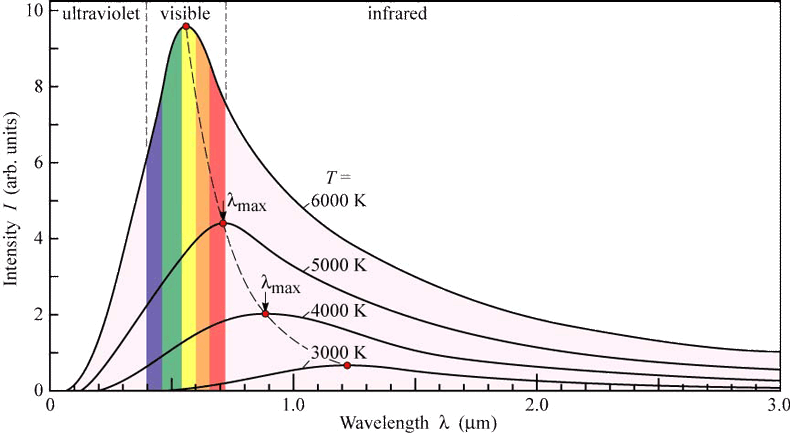
\includegraphics[width=\textwidth]{figures/exampleFigure.png}
		\caption{Portrait figure}
		\label{fig:figure-portrait}
	\end{figure}
	\clearpage
}

\afterpage{
	\begin{sidewaysfigure}
		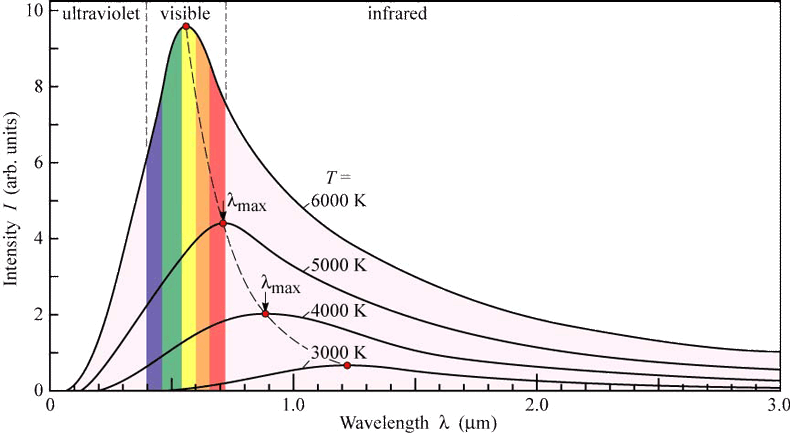
\includegraphics[width=\textwidth]{figures/exampleFigure.png}
		\caption{Landscape figure}
		\label{fig:figure-landscape}
	\end{sidewaysfigure}
	\clearpage
}



%%%%%%%%%%%%%%%%
% Chapter 3
%%%%%%%%%%%%%%%%

\chapter{Results}
\label{chap:results}

Lorem ipsum dolor sit amet, consectetur adipiscing elit, sed do eiusmod tempor incididunt ut labore et dolore magna aliqua. Ut enim ad minim veniam, quis nostrud exercitation ullamco laboris nisi ut aliquip ex ea commodo consequat \cite{ref1}. Duis aute irure dolor in reprehenderit in voluptate velit esse cillum dolore eu fugiat nulla pariatur \cite{ref2}. Excepteur sint occaecat cupidatat non proident, sunt in culpa qui officia deserunt mollit anim id est laborum \cite{ref3}.

\nomenclature{\(c\)}{Speed of light in a vacuum}
\nomenclature{\(h\)}{Planck constant}
\nomenclature{\(\mathbb{R}\)}{Real numbers}
\nomenclature{\(\mathbb{C}\)}{Complex numbers}
\nomenclature{\(\mathbb{H}\)}{Quaternions}

%%%%%%%%%%%%%%%%
% Chapter 4
%%%%%%%%%%%%%%%%

\chapter{Discussion}
\label{chap:discussion}

Lorem ipsum dolor sit amet, consectetur adipiscing elit, sed do eiusmod tempor incididunt ut labore et dolore magna aliqua. Ut enim ad minim veniam, quis nostrud exercitation ullamco laboris nisi ut aliquip ex ea commodo consequat \textcite{ref1}. Duis aute irure dolor in reprehenderit in voluptate velit esse cillum dolore eu fugiat nulla pariatur \textcite{ref2}. Excepteur sint occaecat cupidatat non proident, sunt in culpa qui officia deserunt mollit anim id est laborum \textcite{ref3}.

\nomenclature{\(c\)}{Speed of light in a vacuum}
\nomenclature{\(h\)}{Planck constant}
\nomenclature{\(\mathbb{R}\)}{Real numbers}
\nomenclature{\(\mathbb{C}\)}{Complex numbers}
\nomenclature{\(\mathbb{H}\)}{Quaternions}


%%%%%%%%%%%%%%%%
% Chapter 5
%%%%%%%%%%%%%%%%

\chapter{Conclusion}
\label{chap:conclusion}

Lorem ipsum dolor sit amet, consectetur adipiscing elit, sed do eiusmod tempor incididunt ut labore et dolore magna aliqua. Ut enim ad minim veniam, quis nostrud exercitation ullamco laboris nisi ut aliquip ex ea commodo consequat \textcite{ref1}. Duis aute irure dolor in reprehenderit in voluptate velit esse cillum dolore eu fugiat nulla pariatur \textcite{ref2}. Excepteur sint occaecat cupidatat non proident, sunt in culpa qui officia deserunt mollit anim id est laborum \textcite{ref3}.


%%%%%%%%%%%%%%%%
% Appendices
%%%%%%%%%%%%%%%%

\begin{appendices}

%Some Table of Contents entry formatting
\addtocontents{toc}{\protect\renewcommand{\protect\cftchappresnum}{\appendixname\space}}
\addtocontents{toc}{\protect\renewcommand{\protect\cftchapnumwidth}{7em}}

%Begin individual appendices, separated as chapters

\chapter{Experimental Equipment}
Lorem ipsum dolor sit amet, consectetur adipiscing elit, sed do eiusmod tempor incididunt ut labore et dolore magna aliqua. Ut enim ad minim veniam, quis nostrud exercitation ullamco laboris nisi ut aliquip ex ea commodo consequat. Duis aute irure dolor in reprehenderit in voluptate velit esse cillum dolore eu fugiat nulla pariatur. Excepteur sint occaecat cupidatat non proident, sunt in culpa qui officia deserunt mollit anim id est laborum.

\chapter{Data Processing}
Lorem ipsum dolor sit amet, consectetur adipiscing elit, sed do eiusmod tempor incididunt ut labore et dolore magna aliqua. Ut enim ad minim veniam, quis nostrud exercitation ullamco laboris nisi ut aliquip ex ea commodo consequat. Duis aute irure dolor in reprehenderit in voluptate velit esse cillum dolore eu fugiat nulla pariatur. Excepteur sint occaecat cupidatat non proident, sunt in culpa qui officia deserunt mollit anim id est laborum.

\end{appendices}

%%%%%%%%%%%%%%%%
% References
%%%%%%%%%%%%%%%%
% \nocites

\setlength\bibitemsep{\baselineskip}  %manually set separataion betwen items in bibliography to double space
\printbibliography[title={References}]

\addcontentsline{toc}{chapter}{References}  %add References section to Table of Contents

%%%%%%%%%%%%%%%%
% Summary (Korean)
%%%%%%%%%%%%%%%%

\addcontentsline{toc}{chapter}{국문초록}  %add References section to Table of Contents
\clearpage
\begin{flushleft}
    \Large{
        \textbf{국 문 초 록}\\
    }
\vspace{\baselineskip}
\end{flushleft}

\begin{centering}
    \LARGE{
        \textbf{논 문 제 목} \\
    }
\vspace{\baselineskip}
\end{centering}


\begin{flushright}
    이름 \\
    학과 \\
    일반대학원, 연세대학교
\end{flushright}

Lorem ipsum dolor sit amet, consectetur adipiscing elit, sed do eiusmod tempor incididunt ut labore et dolore magna aliqua. Ut enim ad minim veniam, quis nostrud exercitation ullamco laboris nisi ut aliquip ex ea commodo consequat. Duis aute irure dolor in reprehenderit in voluptate velit esse cillum dolore eu fugiat nulla pariatur. Excepteur sint occaecat cupidatat non proident, sunt in culpa qui officia deserunt mollit anim id est laborum.

\blfootnote{핵심되는 말: 키워드1, 키워드2, 키워드3}
%\pagenumbering{gobble}  %remove page number on summary page


\end{document}
